\section{Internet das coisas}
\label{sec:iot}
A Internet nesta última década tem contribuído de forma significativa na economia e sociedade, deixando como legado uma notável infraestrutura de rede de comunicação. O seu maior disseminador nesse período vem sendo \textit{World Wide Web}(WWW), o qual permite o compartilhamento de informação e mídia de forma global \cite{Chandrakanth:2014}.

A Internet está se tornando cada vez mais persistente no cotidiano, devido, por exemplo, ao crescente número de usuários de dispositivos móveis, os quais possuem tecnologias de conexão com a Internet, as quais cada dia tornam-se mais acessíveis \cite{Chandrakanth:2014}.

Em 2010 havia aproximadamente 1,5 bilhão de PCs conectados a Internet e mais que 1 bilhão de telefones móveis \cite{Sundmaeker:2010}. Segundo Gartner\footnotemark \footnotetext{\url{http://www.gartner.com/newsroom/id/3165317}}, 6,4 bilhões de coisas estarão conectadas até o final de 2016 e, em 2020 esse número atingirá cerca de 20,8 bilhões. A previsão de \cite{Sundmaeker:2010}, a qual dizia que a denominada Internet dos PCs seria movida para o que se chama de Internet das Coisas fica então mais evidente neste atual cenário.

A ideia básica da \textit{Internet of things (IoT)}, traduzido para o português como Internet das Coisas é a presença pervasiva de uma variedade de "coisas ou objetos", tais como RFID tags, sensores, telefones móveis, dentre outros. Os quais, através de esquemas de endereçamento único são capazes de interagir com os outros e cooperar com seus vizinhos para alcançar um objetivo em comum \cite{Atzori:2010}. Outros exemplos de "coisas ou objetos" podem ser pessoas, geladeiras, televisores, veículos, roupas, medicações, livros, passaportes, contanto que possam ser identificadas unicamente e possam se comunicar com as outras coisas e/ou possam ser acessados remotamente por humanos.

Dentre as diversas definições de IoT pode-se citar duas, a primeira define de maneira mais geral \cite{iot2020:2008}, enquanto que a segunda especifica melhor como deve ser o cenário ideal da Internet das Coisas \cite{Sundmaeker:2010}.
\begin{enumerate}
\item \textit{Internet of Things} significa rede mundial de objetos unicamente endereçáveis e interconectados, seguindo os protocolos dos padrões de comunicação.
\item IoT é parte integrante da futura Internet e pode ser definida como uma infraestrutura de rede global dinâmica com capacidades de autoconfiguração baseada nos padrões e interoperabilidade dos protocolos de comunicação onde coisas físicas e virtuais têm identidade, atributos físicos, personalidade virtual, usam interfaces inteligentes e, são integradas dentro da rede de informações.
\end{enumerate}

Diante deste cenário, pode-se citar exemplos de aplicações na IoT para diversos domínios, tais como, logística e transporte; cuidados com a saúde; ambiente inteligente (casa (seção \ref{sec:hns}), escritório); \cite{Atzori:2010} verificação de procedência alimentícia; dentre outros. Seguem dois exemplos de aplicações, uma na área de cuidados com a saúde e outra na verificação de procedência de alimentos, respectivamente.

\begin{itemize}
\item Dispositivos implantáveis com capacidade de comunicação sem fio podem ser utilizados para armazenar registros sobre a saúde de um paciente em situações de risco e podem ser decisivos para salvar a vida do paciente. A capacidade de ter acesso a essas informações nessas circunstâncias fazem com que hospitais possam saber de imediato como tratar um paciente que esta a caminho. Esta possibilidade é especialmente útil para pessoas com diabetes, câncer, problemas de coração na artéria coronária, doenças do pulmão, assim como as pessoas com implantes médicos complexos, tais como, marcapassos, tubos, transplantes de órgãos e aqueles que podem ficar inconscientes e incapazes de comunicar-se durante uma operação \cite{Weber:2010}.
\item Rastreabilidade de produtos alimentícios ajudam os usuários a verificar a origem de um produto, assim como informações de composição química, dentre outros. Mas também previne de doenças não desejadas. Por exemplo, avisos atuais sobre a mercadoria em questão podem ser disponibilizados à medida que o produto sai da origem e vai passando para os outros níveis de consumo, desta forma os consumidores podem evitar o contágio de doenças como gripe aviária e, encefalopatia espongiforme bovina (EEB), mais conhecida como doença da vaca louca \cite{Weber:2010}.
\end{itemize}

Apesar da grande potencialidade da Internet das Coisas, a qual gerou em 2015 um faturamento em torno de 130,33 bilhões de dólares americanos e tem prospecção de chegar até 883.55 bilhões em 2020\footnotemark \footnotetext{http://www.marketsandmarkets.com/Market-Reports/iot-application-technology-market-258239167.html}, ainda existem muitos desafios a serem vencidos, tais como segurança da informação, armazenamento e processamento de grande quantidade de dados, dentre outros. Adentrando um pouco em um dos desafios da IoT, o da disponibilidade de uma interface de comunicação (acesso aos serviços e informações dos dispositivos) e programação comum aos objetos, pode-se dizer que a falta desta padronização faz com que se torne oneroso o desenvolvimento de aplicações para o objeto. Mais difícil ainda é prover uma única funcionalidade ou serviço com a composição dos diversos objetos. Para diminuir a dificuldade deste cenário, pode-se disponibilizar os dispositivos como serviços Web (seção \ref{subsec:dispositivosWeb}), assim sendo se pode utilizar os protocolos Web como linguagem comum de integração dos dispositivos a Internet \cite{Franca:2011}.

\subsection{Serviços Web}
\label{ws:webservices}
Segundo \cite{Dustdar:2005}, um serviço Web é um sistema identificado por uma URL\footnotemark \footnotetext{Acrônimo para Uniform Resource Locator e é uma referência (um endereço) para um recurso na Internet.\url{https://docs.oracle.com/javase/tutorial/networking/urls/definition.html}}, no qual suas interfaces públicas são definidas e descritas usando XML\footnotemark \footnotetext{Extensible Markup Language (XML) é uma simples e flexível linguagem de marcação utilizada para codificar documentos através de regras produzidas por humanos, as quais podem ser manipulados (compreendidas) por máquinas \cite{w3c:xml}, \cite{w3c:xmlschema}} e, suas definições são padronizadas e podem ser descobertas por outros sistemas. Sistemas então podem interagir com os serviços Web utilizando suas definições e descrições. Mensagens XML são transmitidas seguindo os protocolos padrão (definidos por W3C\footnotemark \footnotetext{\url{https://www.w3.org/}}) da Internet para que haja tal interação.

Serviços Web surgiram tendo como principal foco o reúso de aplicações existentes (dentre as quais incluíam código fonte legado) para que pudessem se integrar de forma leve com outras aplicações. Geralmente essa integração tinha como referência o desejo de  novas formas de compartilhamento dos serviços ao longo das diversas linhas do negócio ou entre parceiros. Como exemplo, considere o cenário da Figura \ref{fig:ws_purchase_order} o qual demonstra a utilização de diferentes serviços (\textit{Credit service, Inventory service, Billing service, Shipmente service}) para prover um único serviço, pedido de uma ou mais mercadorias, ambiente comum do E-Commerce.

\begin{figure}[!htb] \centering 
  \centering
  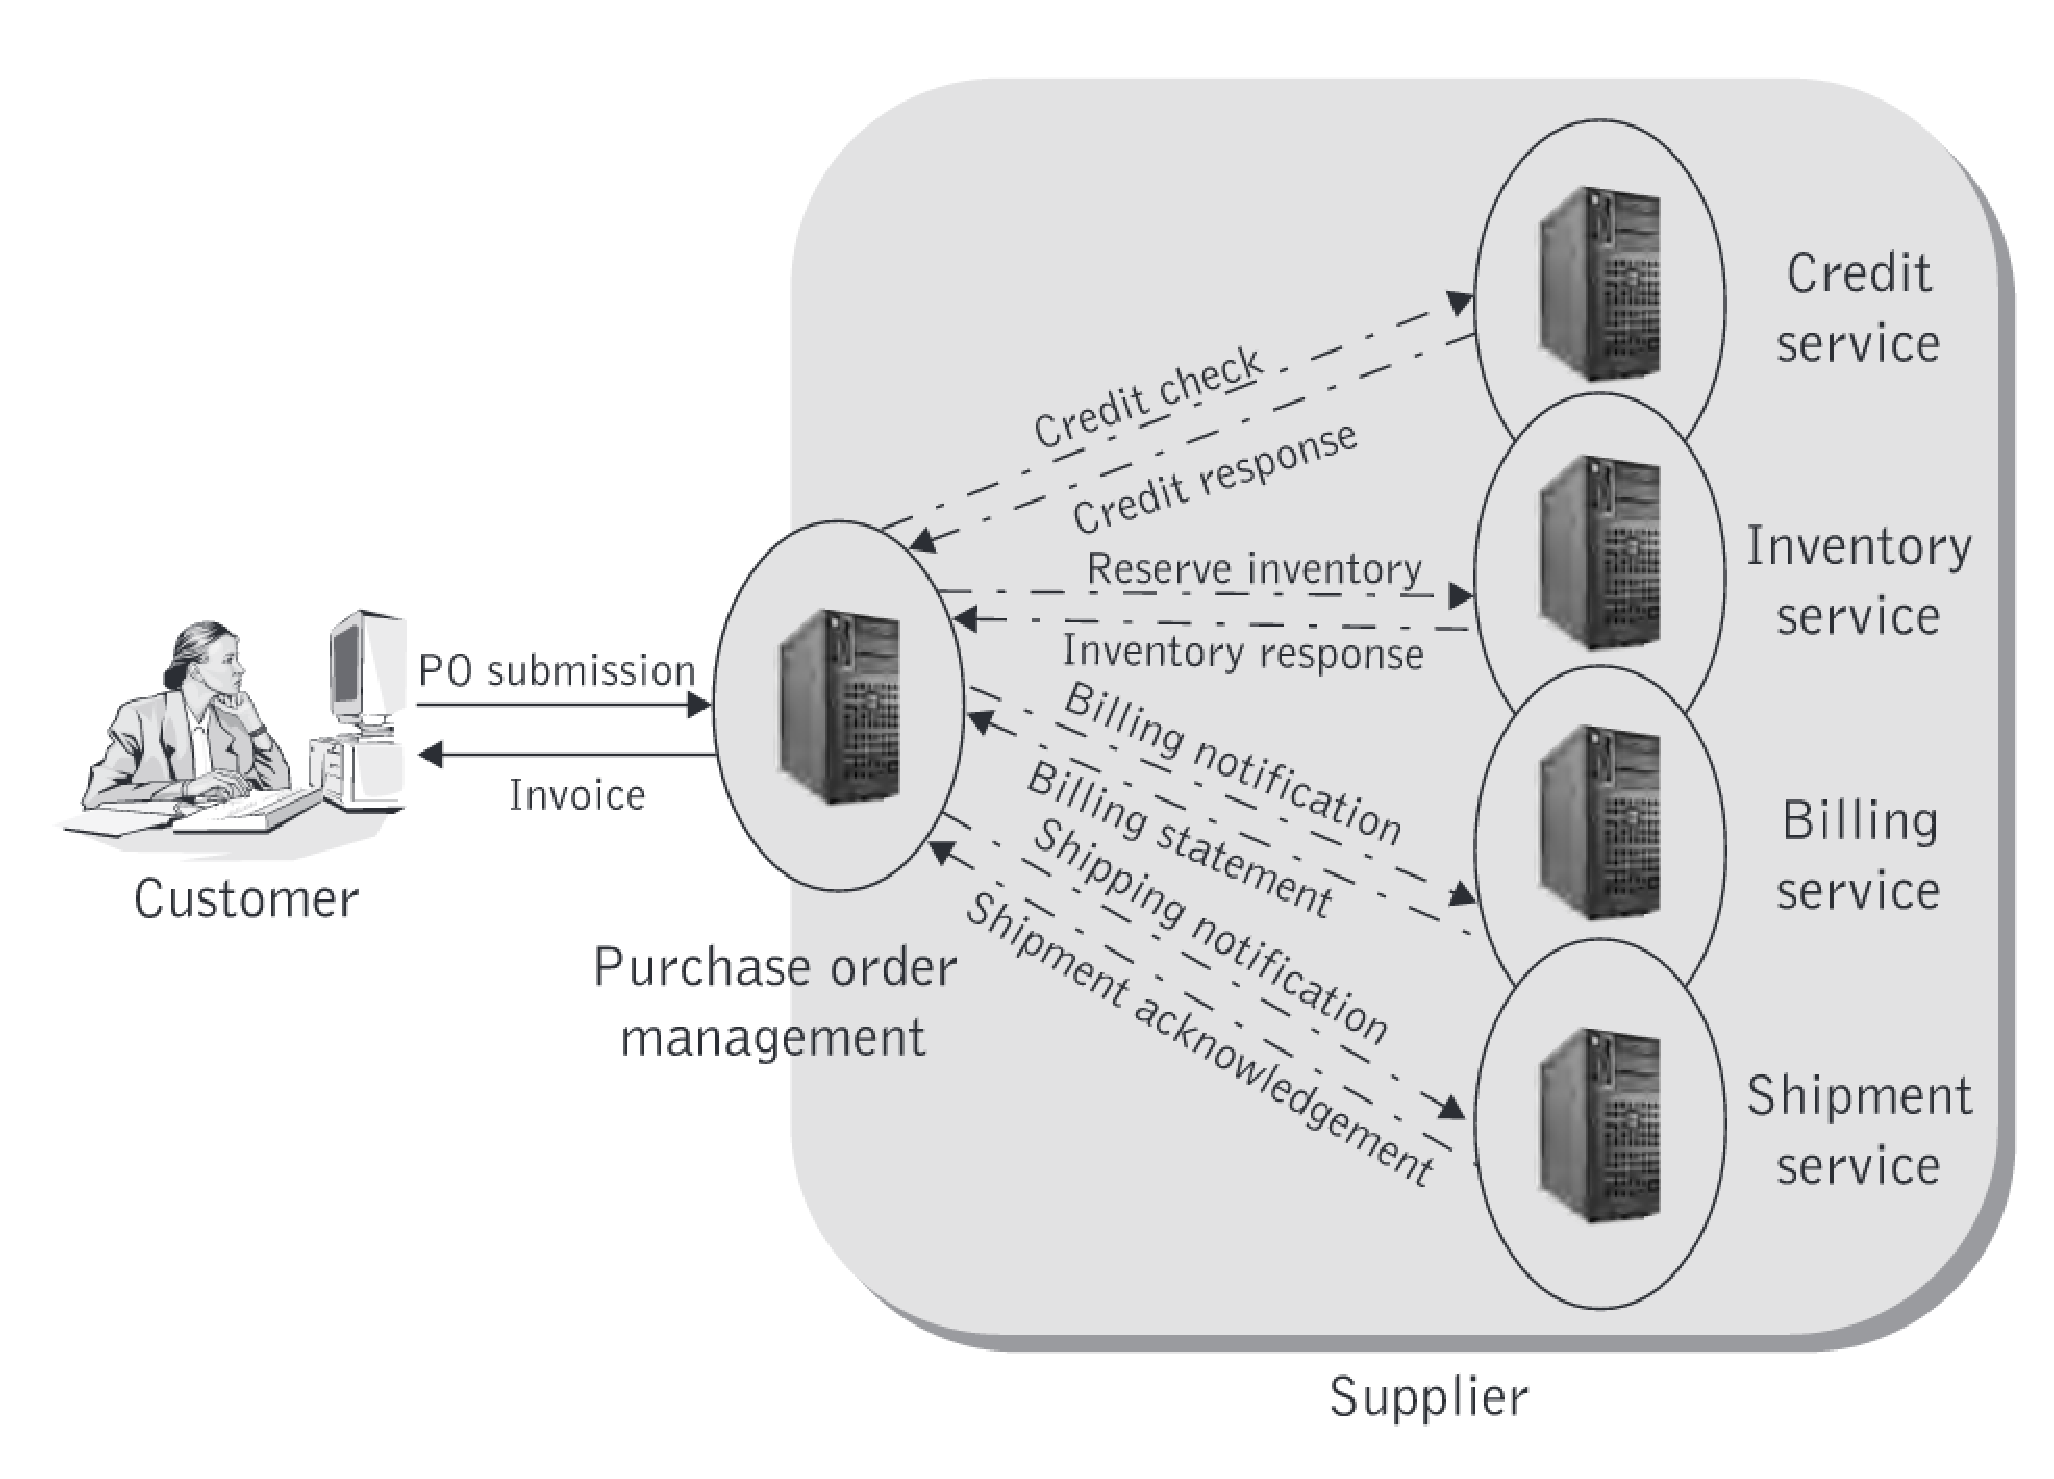
\includegraphics[width=0.8\columnwidth]{fundamentacao/webservice_purchase_order} 
  \caption{Utilização de diferentes serviços Web para prover o serviço de pedido de um E-Commerce. \cite{Papazoglou:2008}} 
  \label{fig:ws_purchase_order}
\end{figure}

Serviços Web possuem algumas características:
\begin{enumerate}
\item Podem ser ditos \textit{stateless} (sem estado) ou \textit{stateful} (com estado). Se um serviço pode ser invocado repetidamente sem ter que manter um contexto ou estado este é denominado \textit{stateless}. Como exemplo de serviço \textit{stateless} pode-se citar a recuperação de informação de um sensor de temperatura, pois não precisa de nenhum tipo de memória para manter o que aconteceu durante as requisições ao serviço. Já os serviços que precisam manter seus contextos preservados de uma invocação para a próxima requisição, estes são \textit{stateful}. Por exemplo, um usuário quando chama um serviço (Levar compras) de um \textit{Home Network Service} (ver seção \ref{sec:hns}), este então começa sua execução: um veículo (um serviço) leva a carga até uma determinada área próxima ao elevador (um serviço) e, uma garra mecânica (um serviço) pega a carga e coloca dentro do elevador. Observe que o serviço Levar compras é a composição de diferentes serviços e não pode ser chamado e executado diversas vezes continuamente sem a necessidade de manter seu contexto entre os diferentes serviços envolvidos, pois o ambiente não tem mais de um carro, mais de uma garra e elevador. Então a menos que este já tenha terminado toda a sua execução, poderia ser chamado e executado novamente. Por tal motivo este serviço mantêm um estado (em execução ou sem trabalho) o qual depende dos estados dos serviços envolvidos \cite{Papazoglou:2008}.
\item Podem ser ditos com baixo nível de acoplamento (\textit{loose coupling}) quando os serviços interagem uns com os outros e utilizam-se as tecnologias padrões da Internet, permitindo dessa forma construir pontes entre sistemas que de outra forma exigiriam grandes esforços de desenvolvimento de software. O termo acoplamento indica o nível de dependência entre serviços \cite{Papazoglou:2008}.
\item Podem ser ditos síncronos e assíncronos. Quando síncrono, clientes realizam suas requisições e ficam sempre aguardando uma resposta. O cliente é dependente de tal resposta para continuar sua computação. Se uma operação for incapaz de ser completada, o resto da computação é impedida de continuar. Enquanto que nos assíncronos o cliente não necessita aguardar uma resposta para continuar a execução de sua aplicação. Quando um cliente invoca um serviço assíncrono, o cliente normalmente envia um documento inteiro, como uma ordem de pagamento ou, uma lista de itens de um carrinho de compra com o tipo de pagamento e endereço de entrega. O serviço aceita o documento inteiro e processa-o, podendo retornar ou não uma mensagem de resultado. A resposta do serviço, se existir alguma, pode acontecer horas ou talvez dias depois \cite{Papazoglou:2008}.
\end{enumerate}

Serviços Web possuem baixo nível de acoplamento e utilizam padrões para oferecer suas funcionalidades, pois tais serviços tem a intenção de prover comunicação a diferentes tipos de aplicações, que possivelmente são executadas em diferentes plataformas. A \textit{Web Service Description Language}(WSDL) usa o formato XML para descrever os métodos oferecidos por um serviço Web, incluindo parâmetros de entrada e saída, tipos de dados e, protocolo de transporte utilizado (normalmente o HTTP). Além de informações referente ao provedor do serviço, tais como, endereço e contato da empresa desenvolvedora do serviço. O \textit{Simple Object Access Protocol}(SOAP, seção \ref{subsec:soap}) é utilizado para as trocas de mensagens (formatadas em XML) entre as entidades envolvidas no modelo de serviço Web citado\cite{Dustdar:2005}, como pode ser visto na Figura \ref{fig:wsmodelsoap} e explicado logo abaixo. Esse tipo de serviço Web é chamado de serviço Web baseado em SOAP \cite{Belqasmi:2011}.

\begin{figure}[!htb] \centering 
  \centering
  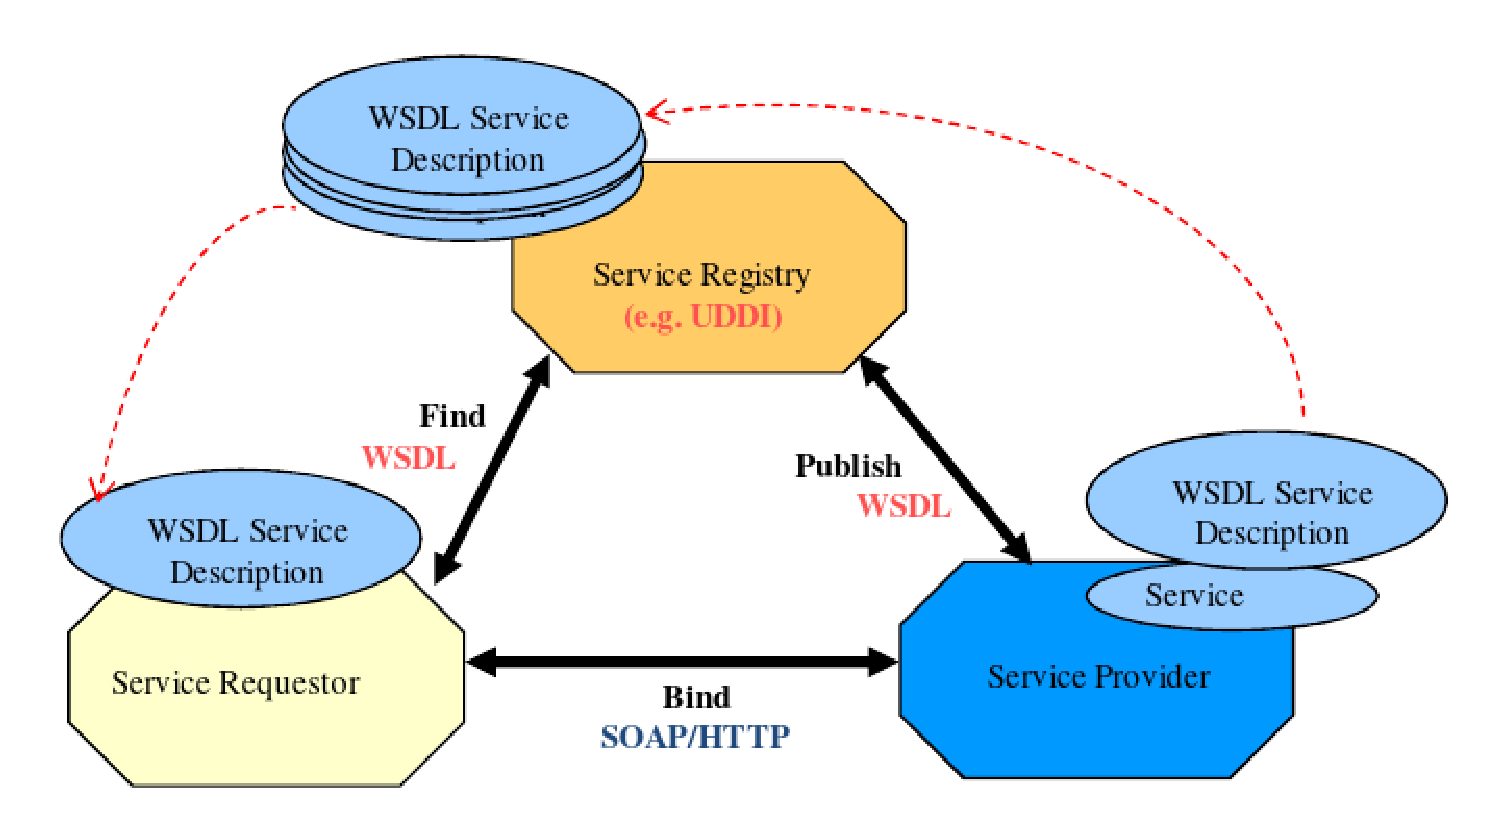
\includegraphics[width=0.8\columnwidth]{fundamentacao/webservice_soap_model} 
  \caption{Modelo de serviço Web baseado em SOAP. \cite{Belqasmi:2011}} 
  \label{fig:wsmodelsoap}
\end{figure}

\begin{itemize}
\item Provedor (Service Provider) - cria e oferece o serviço Web, este precisa descrever o serviço em um formato padrão, neste caso WSDL e, publica-o (\textit{Publish}) no Registro de serviço.
\item Registro de serviço (Service Registry) - contém a descrição publicada pelo Provedor. O registro de serviço mais utilizado é o \textit{Universal Description, Discovery and Integration} (UDDI), este em suas especificações define um conjunto de \textit{Application Program Interfaces}(APIs) tanto para publicação, quanto para descoberta \cite{Belqasmi:2011}.
\item Consumidor (Service Requestor) - obtém informações do registro, \textit{Find}, e utiliza a descrição do serviço capturada para invocar (\textit{Bind}) o serviço Web.
\end{itemize}

A descrição realizada da Figura \ref{fig:wsmodelsoap} foi na verdade a descrição das 3 regras fundamentais do Service Oriented Architecture (SOA), que é um caminho lógico para projetar sistemas de software, os quais podem prover serviços tanto para o usuário final de aplicações quanto para outros serviços distribuídos na rede, através de interfaces que possam ser publicadas e descobertas \cite{Papazoglou:2008}.

Existe também outro tipo de abordagem de serviços Web, baseada nos princípios arquiteturais REST (ver seção \ref{subsec:restful}).

\subsection{SOAP}
\label{subsec:soap}
SOAP é um protocolo leve que foi desenvolvido com a intenção de prover troca de mensagens estruturadas em um ambiente descentralizado e distribuído. Este usa a tecnologia XML para definir um framework extensível de mensagens, o qual permite a construção de mensagens que podem ser trocadas através de uma variedade de protocolos subjacentes. O framework foi desenvolvido para ser independente de modelo de linguagem de programação ou qualquer outra implementação semântica \cite{w3c:soap}. Diz-se que é um protocolo leve pelo fato de somente receber e enviar pacotes de protocolos de transportes (por exemplo, HTTP) e, processar as mensagens XML, quando contrastados com os protocolos ORPC \cite{Papazoglou_slides:2008}. A figura \ref{fig:wsmodelsoap_expanded} seguinte mostra como o SOAP atua no modelo de serviço Web baseado em SOAP (Figura \ref{fig:wsmodelsoap}). Nesta, o \textit{SOAP-based middleware} converte as chamadas de procedimento de/para mensagens XML que são enviadas através do HTTP ou outro protocolo.

\begin{figure}[!htb] \centering 
  \centering
  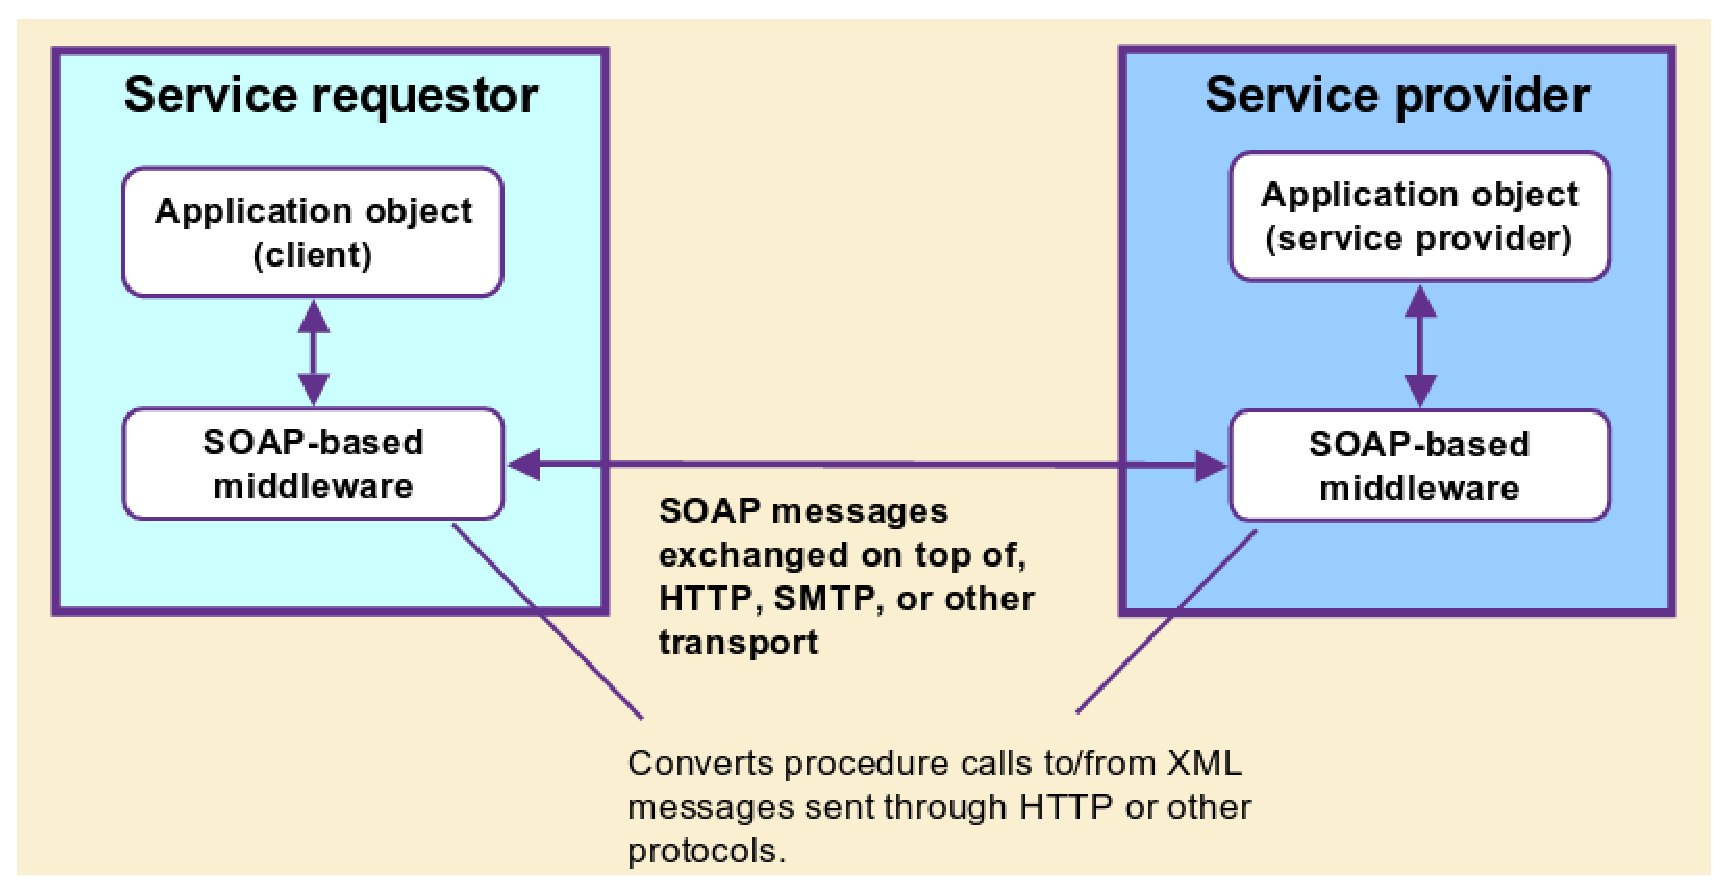
\includegraphics[width=0.8\columnwidth]{fundamentacao/webservice_soap_model_expanded} 
  \caption{SOAP no modelo Modelo de serviço Web baseado em SOAP. \cite{Papazoglou_slides:2008}} 
  \label{fig:wsmodelsoap_expanded}
\end{figure}

Em outras palavras, SOAP é um protocolo (da camada de aplicação) utilizado para transferir mensagens entre instâncias de serviços descritas por interfaces WSDL (ver Figura \ref{fig:wsmodelsoap_communication_msg}).

\subsection{Serviços Web RESTFul}
\label{subsec:restful}
Segundo \cite{Heffelfinger:2014}, Representational State Transfer (REST) é um estilo de arquitetura no qual serviços Web são vistos como recursos e podem ser identificados por Uniform Resources Identifiers (URIs). Serviços Web que são desenvolvidos usando REST são conhecidos como RESTful web services. 

Os principais princípios do estilo arquitetural REST são: endereçamento global através de identificação dos recursos, interface uniforme compartilhada por todos os recursos, interações \textit{stateless} entre os serviços e, mensagens auto-descritivas e \textit{hypermedia} como um mecanismo para descoberta descentralizada de recursos por referência \cite{Pautasso:2014}, conforme abaixo.

\begin{enumerate}
\item Identificação dos recursos - todos os recursos que são publicados por um serviço Web deveriam ser disponibilizados por um único e estável identificador global \cite{Pautasso:2014}. A exemplo das URIs \cite{Franca:2011}.
\item Interface uniforme - todos os recursos interagem através de uma interface uniforme, a qual prover um conjunto de métodos pequeno, genérico e funcionalmente suficiente para suportar todas as possíveis interações entre os serviços. Cada método tem uma semântica bem definida em relação aos efeitos que causará no estado do recurso. No contexto da Web e do protocolo HTTP que é utilizado, ``Interface uniforme'' pode ser alcançado com os seus  métodos (GET, PUT, DELETE, POST, HEAD, OPTIONS, dentre outros) os quais podem ser aplicados para todos os identificadores dos recursos Web (URIs) \cite{Pautasso:2014}.
\item Interações \textit{stateless} - os serviços não podem estabelecer sessões permanentes entre eles. Isto assegura que as requisições para um recurso sejam independentes entre si. No final de cada interação, não há estados compartilhados entre clientes e servidores. Requisições podem resultar em uma mudança de estado do recurso, mas o novo estado é imediatamente visível para todos clientes \cite{Pautasso:2014}.
\item Mensagens auto-descritivas - Serviços interagem através de requisição e mensagem de resposta, que contem tanto os dados (representações dos recursos) e correspondente \textit{meta-data}. As representações podem variar de acordo com o contexto do cliente, interesses e habilidades. Por exemplo, um cliente \textit{mobile} pode obter uma representação do recurso que exige pouco consumo de banda de dados. Da mesma forma, um navegador pode requisitar a representação de uma página Web em uma linguagem específica, de acordo com suas preferências. Esta característica aumenta de maneira significativa o grau de interoperabilidade, pois um cliente pode dinamicamente negociar o mais apropriado formato de representação com o recurso (também conhecido como media type), em vez de ser forçado a sempre trabalhar com uma determinada representação do recurso. As requisições e mensagens de respostas também devem conter explicitamente \textit{meta-data} sobre sua representação, desta maneira os serviços não precisam assumir algum tipo de acordo de sobrecarga no sentido de como tal representação seria analisada, processada e entendida \cite{Pautasso:2014}.
\item \textit{Hypermedia} - Recursos podem ser relacionados entre si. \textit{Hypermedia} embute referências a outros recursos relacionados ou dentro de suas representações ou em sua correspondente \textit{metadata}. Clientes então podem descobrir os \textit{hyper-links} dos recursos relacionados ao processar suas representações e escolher seguir o link. Como exemplificado em \cite{Franca:2011}, um sistema de uma instituição que possui um recurso lista\_cursos (lista todos os cursos da instituição), este pode oferecer os \textit{hyper-links} que representam cada recurso que representa um determinado curso. \textit{Hypermedia} auxilia na descoberta descentralizada de recursos e também pode ser utilizada para descoberta e descrição de protocolos de interação entre os serviços. Pelo fato deste ser o princípio menos utilizado pelas APIs que se dizem ser RESTFul, algumas vezes as APIs disponibilizadas por serviços Web que além das outras restrições contemplam esta, são também chamadas de \textit{Hypermedia APIs} \cite{Pautasso:2014}.
\end{enumerate}

\subsection{Dispositivos como serviços Web RESTFul} 
\label{subsec:dispositivosWeb}
Como abordado em \ref{sec:iot} um dos desafios referentes a visão da IoT é sua interoperabilidade e, como possível solução se pode disponibilizar os dispositivos como serviços Web, neste caso seguindo os príncipios REST. Desta maneira os dispositivos podem interagir entre si e com outros sistemas na Web.

A disponibilização dos dispositivos como serviços Web RESTFul vêm sendo empregada através de duas abordagens. Na primeira, quando os dispositivos têm recursos suficientes (memória, processamento e largura de banda de rede) servidores Web são embarcados nos próprios dispositivos e estes são disponibilizados como recursos REST. Enquanto que na segunda, quando uma coisa não possui recursos suficientes para tal propósito, utiliza-se de outro dispositivo, por exemplo, um \footnotemark{Raspberry Pi}\footnotetext{https://www.raspberrypi.org/products/} ou qualquer outro controlador com recursos suficientes para instalação e execução de um servidor Web. Este então atua como um intermediador entre o objeto e a Internet \cite{Franca:2011}.

Adotando esse padrão, os dispositivos podem ter suas propriedades disponíveis através de qualquer navegador, sem a necessidade de instalação de nenhum programa ou driver adicional, como pode ser exemplificado na Figura \ref{fig:dispnavegador}. Além disto, mashups físicos\footnotemark \footnotetext{Aplicativos criados a partir da composição de dados e serviços de dispositivos físicos com outros recursos Web.} podem ser construídos com muito menos esforço do que as existentes abordagens, minimizando a barreira para o desenvolvimento de aplicações com dispositivos \cite{Guinard:2009}. Pelo fato das coisas serem disponibilizadas como serviços Web, ainda pode-se utilizar-se dos outros recursos disponíveis na Web, a exemplo de sistemas de cache, balanceamento de carga, indexação e pesquisa \cite{Franca:2011}. Assim então promovendo a visão da Internet das Coisas.

\begin{figure}[!htb] \centering 
  \centering
  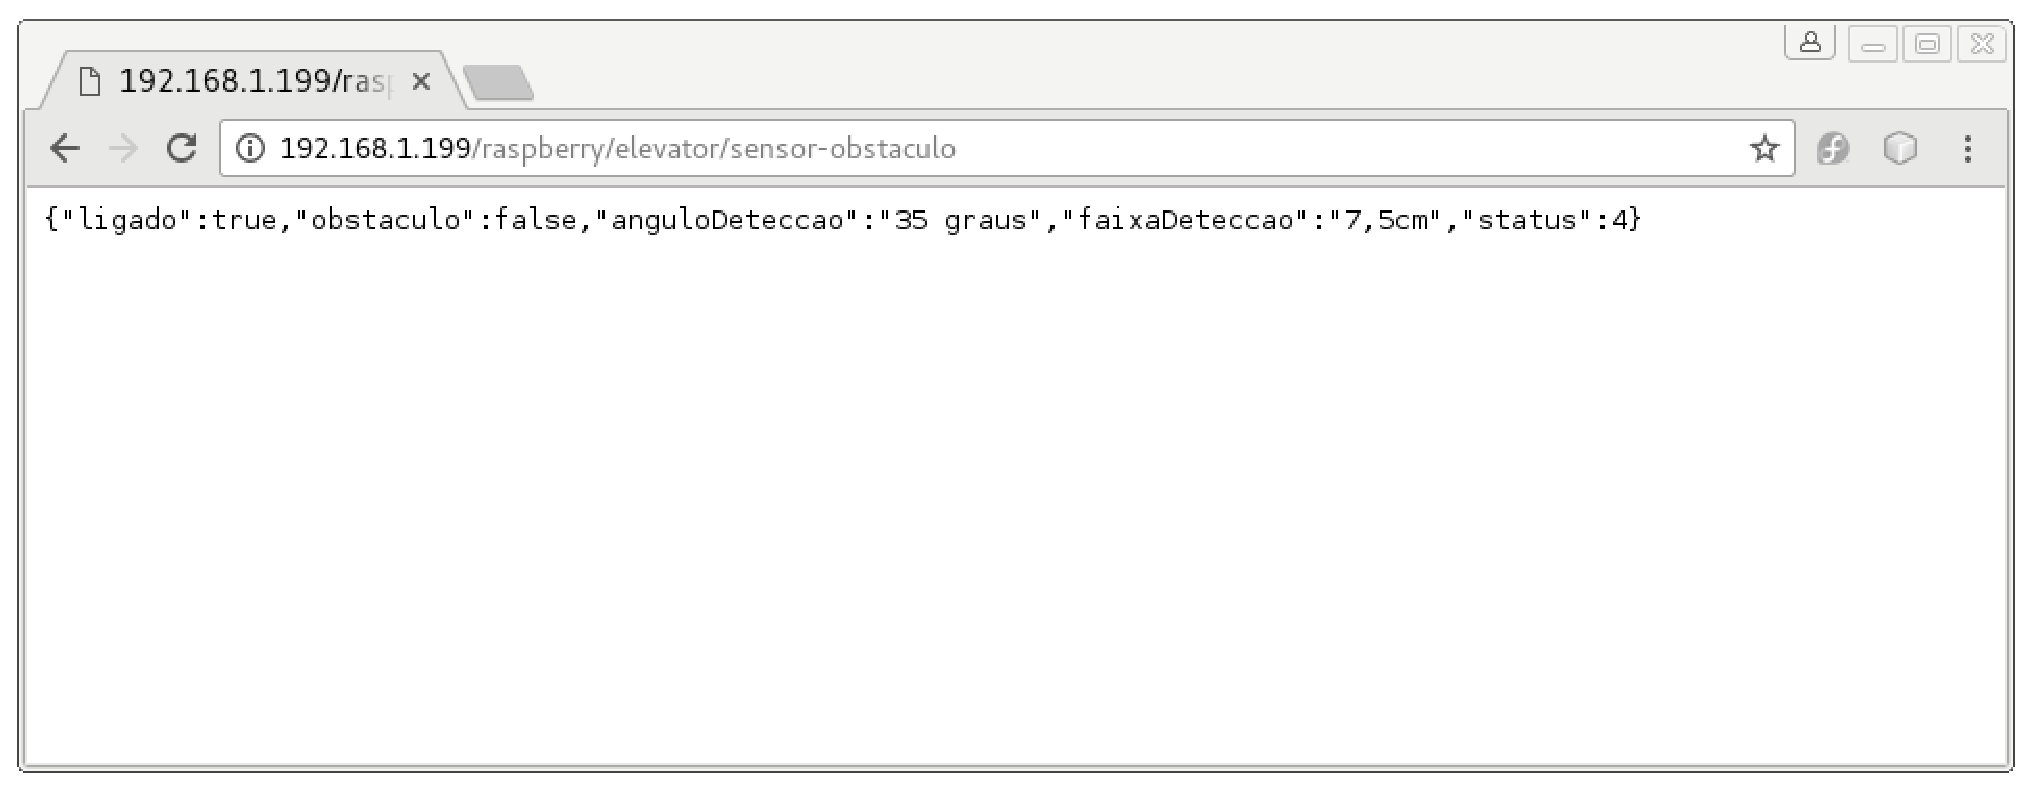
\includegraphics[width=0.8\columnwidth]{fundamentacao/elevator_sensor_example} 
  \caption{Dispositivo sensor de obstáculo do elevador disponibilizado como serviço. Faixa de detecção compatível com a largura do elevador utilizado na maquete do cenário (Figura \ref{fig:cenario_real})} 
  \label{fig:dispnavegador}
\end{figure}

No cenário da IoT os princípios REST têm sido amplamente aplicados na integração dos dispositivos inteligentes a Web, pois esses princípios parecem ser mais adequados para dispositivos com poucos recursos de hardware \cite{Franca:2011}. Para deixar claro os motivos da adoção do REST para disponibilização de dispositivos como serviços Web ao invés dos serviços Web baseados em SOAP, será realizada uma comparação a seguir.

Uma das diferenças entre o REST e WS-* SOAP está na forma como o protocolo HTTP é empregado. Com REST, o HTTP é utilizado para prover interfaces uniformes onde cada método (GET, PUT, DELETE, POST, HEAD, OPTIONS, dentre outros) tem uma semântica bem definida em relação aos efeitos que causará no estado do recurso \cite{Franca:2011}, enquanto que nos WS-* SOAP cada serviço tem seu próprio conjunto de operações explicitamente declarados dentro de um documento WSDL \cite{Pautasso:2014}. O SOAP utiliza o HTTP como um protocolo de transporte (HTTP é um protocolo da camada de aplicação de rede). As mensagens SOAP são adicionadas ao corpo do HTTP. Nos WS-* SOAP o método POST do HTTP é utilizado na troca de mensagens entre cliente e servidor e, a informação sobre qual funcionalidade deve ser executada está presente na mensagem SOAP e não na requisição HTTP. Os serviços Web baseados em SOAP utilizam a Web como meio de troca de mensagens, enquanto os serviços Web RESTFul são parte da Web, ou seja, é visto como um terreno comum para as aplicações \cite{Franca:2011}.

O formato da mensagem SOAP ocasiona um maior consumo de banda devido ao tamanho da mensagem SOAP (ver Figura \ref{fig:msg_soapXrest}), um dos principais motivos para utilizar dispositivos como serviços Web RESTFul, pois muitos dispositivos na IoT possuem baixa capacidade de processamento e de banda de rede. Além disso, este formato pré-definido de mensagem força o cliente a tratar sempre este tipo de mensagem, enquanto utilizando REST é possível oferecer diferentes tipos de representações (JSON, XML, dentre outros) \cite{Franca:2011}.

\begin{figure}[!htb] \centering 
  \centering
  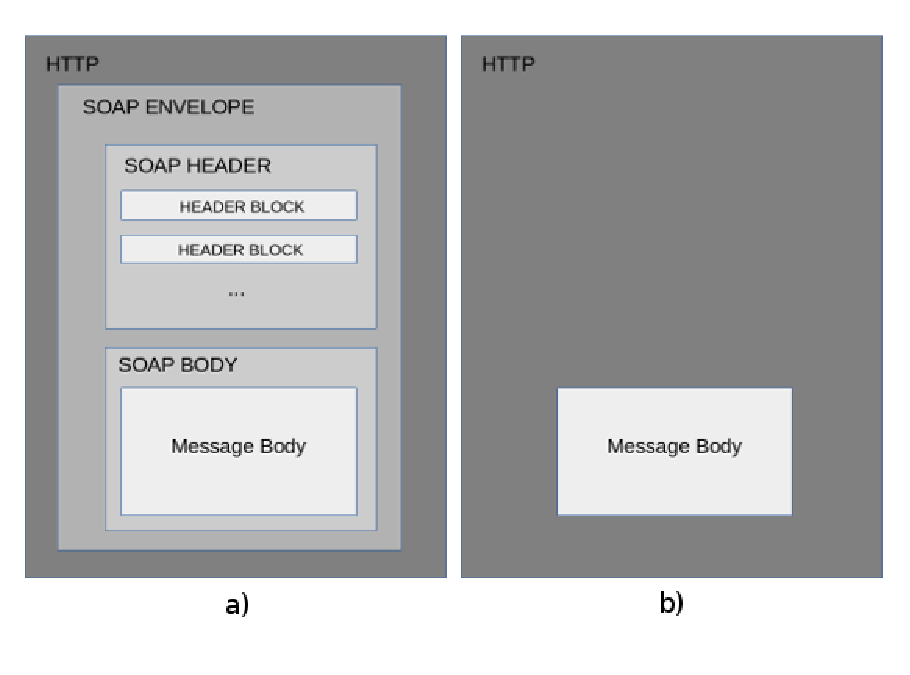
\includegraphics[width=0.8\columnwidth]{fundamentacao/messages_restXsoap} 
  \caption{a)Mensagem SOAP sobre HTTP. b)Mensagem utilizando REST sobre HTTP. Figura baseada em \cite{Pautasso:2014}.}
  \label{fig:msg_soapXrest}
\end{figure}

Em relação ao termo ``fraco acoplamento'', o mesmo se refere a capacidade de fazer modificações no provedor de serviço sem afetar o cliente, os serviços Web RESTFul são menos acoplados, pois as operações sobre os recursos não mudam, já que tais operações são sobre os métodos do HTTP. Uma ressalva é que se as alterações forem feitas nos parâmetros passados nas mensagens, tanto o SOAP quanto o REST estarão no mesmo nível de acoplamento \cite{Franca:2011}.

Por fim, na Figura \ref{fig:comparative_services_soap_rest} é apresentado uma análise comparativa entre duas aplicações que oferecem as mesmas funcionalidades, sendo que uma foi construída utilizando serviços Web SOAP e a outra utilizando serviços Web baseado nos princípios arquiteturais REST. A aplicação em questão é de conferência multimídia e pode ser usada para criar uma conferência, adicionar ou remover um participante de uma conferência que esteja em progresso, atualizar o tipo de mídia (mudar de audio para vídeo) e deletar uma conferência. Ambas as aplicações foram desenvolvidas em um mesmo ambiente e foram publicadas em um mesmo servidor de aplicação. Vários cenários foram executados e performances foram medidas. Todas as medidas são de tempo (milissegundos) e cada resultado é a média de 10 experimentos. Observe que tanto na mesma máquina quanto em um ambiente distribuído a performance do REST é sempre melhor, sendo superior de 3 até 5 vezes em relação ao SOAP quando em ambiente distribuído \cite{Belqasmi:2012}.

\begin{figure}[!htb] \centering 
  \centering
  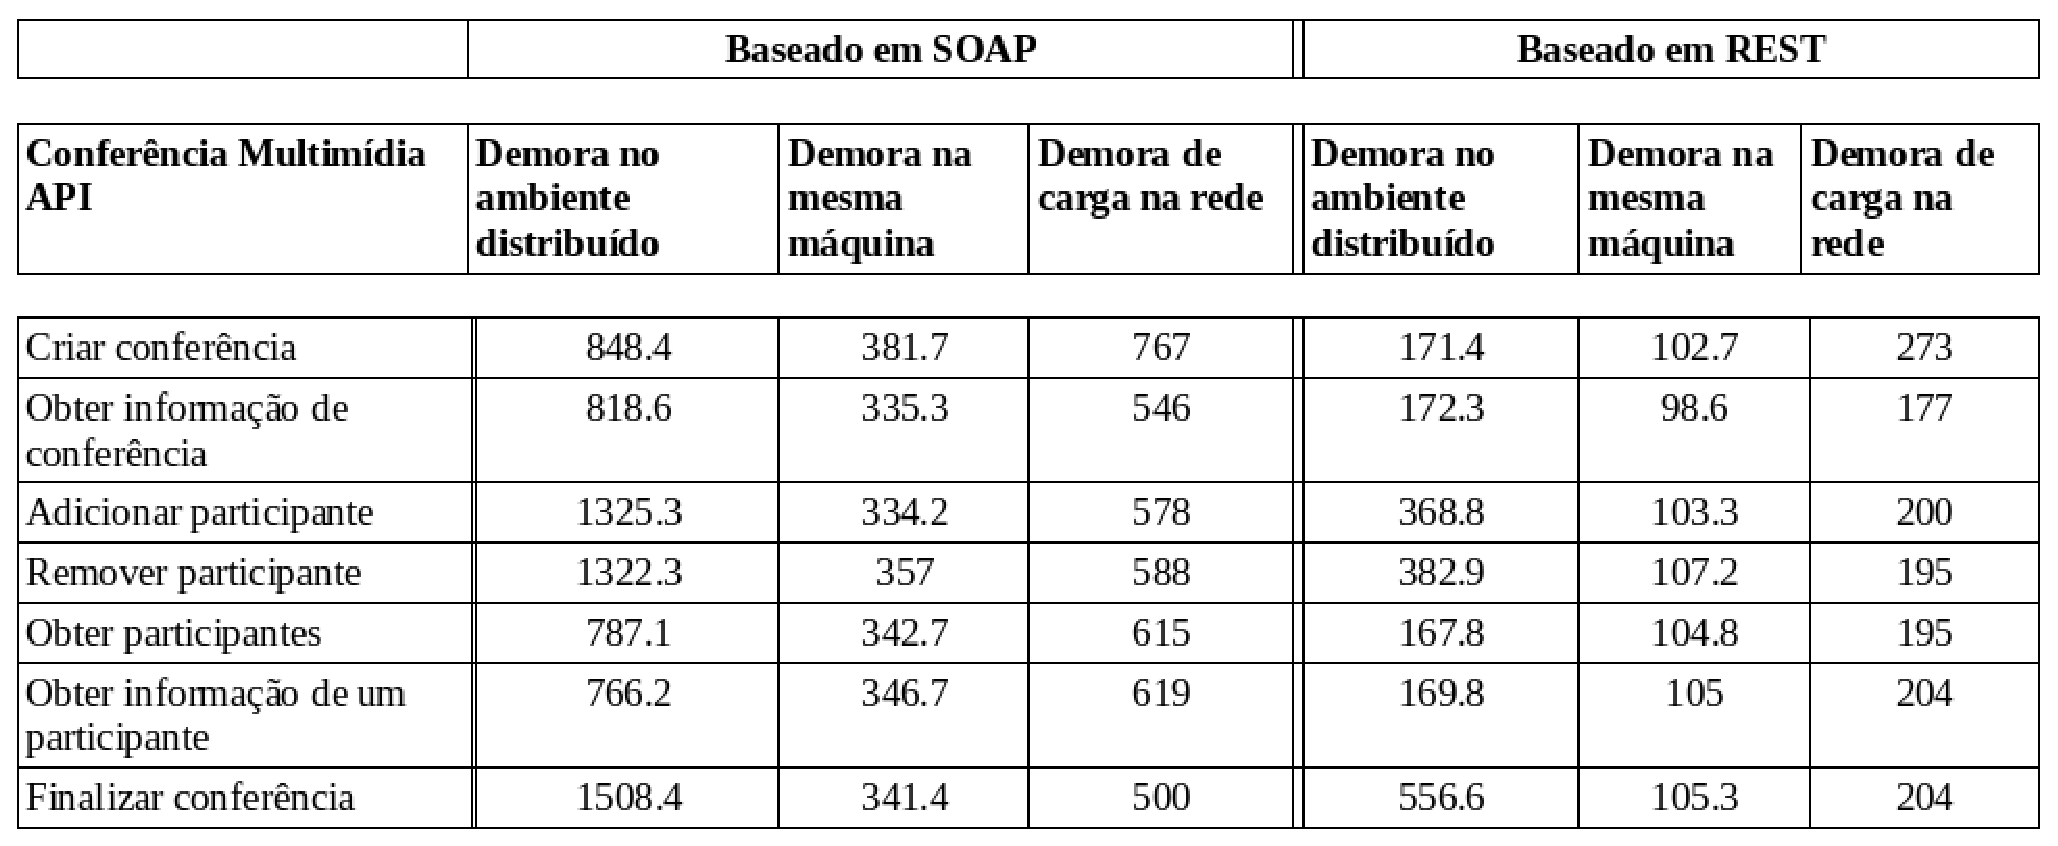
\includegraphics[width=0.8\columnwidth]{fundamentacao/comparative_services_soap_rest} 
  \caption{Resultados de performance entre duas aplicações com mesmas funcionalidades, mas uma baseada em SOAP e outra em REST. Figura adaptada de \cite{Belqasmi:2012}.}
  \label{fig:comparative_services_soap_rest}
\end{figure}

Diante do cenário da IoT descrito até agora faz-se observar que muitos objetos quando isolados, não têm como prover funcionalidade(s) que atendam ao(s) requisito(s) de um usuário final (outra coisa ou um humano). Então, para atender a tais requisitos, há necessidade de compor estes objetos com outros para oferecer nova(s) funcionalidade(s) que atendam aos usuários finais. Entretanto, a composição das coisas pode levar a uma interação de caracterı́sticas (seção \ref{sec:featureinteraction}) a qual pode provocar efeitos colaterais indesejáveis.

\section{Interação de características}
\label{sec:featureinteraction}
Em desenvolvimento de \textit{software}, uma \textit{feature} (característica) é um componente de adicional funcionalidade ao \textit{software} \cite{Calder:2003}, consistindo de um conjunto de requisitos logicamente relacionados e suas especificações, o qual se destina a fornecer um determinado efeito comportamental \cite{NHLABATSI:2008}.

Poucas \textit{features} atendem aos requisitos do usuário final quando estão isoladas. Para resolver este problema, características são combinadas para fornecer um novo componente de funcionalidade ao software. Entretanto, quando a composição de \textit{features} leva a algum comportamento não esperado - interação de características, esta pode resultar em efeitos colaterais indesejáveis \cite{NHLABATSI:2008} ou em efeitos colaterais desejáveis \cite{Weiss:2005}.

Efeito colateral indesejável é quando há interação de características e esta resulta em um estado inconsistente do sistema, um sistema instável ou dados imprecisos. Já efeito colateral desejável é quando a interação de características resulta num comportamento que ajudará de algum modo a funcionalidade em questão \cite{Weiss:2005}, \cite{NHLABATSI:2008}.

Existem diversas causas para interação de características, algumas delas são listadas a seguir de forma mais genérica possível \cite{Weiss:2007}.

\begin{itemize}
\item \textit{Goal Conflit} (Conflito de interesses): Cada característica tem seus próprios objetivos (designadas para fazer algum tipo de processamento, coletar algum dado, dar uma saída específica, dentre outros) a serem alcançados. Entretanto, quando as características são combinadas, os objetivos das duas características podem entrar em conflito e não se pode garantir que todos sejam alcançados. 
\item \textit{Resource Contention} (Contenção de recurso): \textit{Features} podem estar competindo umas com as outras devido ao acesso a recursos de capacidade limitada, tais como, memória, CPU, largura de banda, acesso a banco de dados, dentre outros. Desta forma, a correta execução de uma característica pode ser comprometida por outra característica que esteja utilizando além da sua cota de um recurso compartilhado.
\item \textit{Violation of Assumptions} (Violação de suposições): Desenvolvedores das funcionalidades de software precisam fazer algumas suposições de como outras características trabalham. Estes podem fazer suposições incorretas, por exemplo, devido a semântica ambígua (tal como uso do mesmo conceito de diferentes formas), ou devido a presença de diferentes versões da mesma funcionalidade de software. De forma similar, implementação de características podem ser baseadas em suposições incorretas sobre o contexto de uso. A caracterização de uma  \textit{Violation of Assumptions} se dá quando a mudança em uma \textit{feature} quebra a suposição correta que a outra característica tinha sobre esta.
\item \textit{Policy Conflict} (Conflito de políticas): Políticas proveem os meios para especificação e modularização do comportamento de uma característica, na medida em que alinha suas capacidades e restrições com os requisitos de seus usuários. A \textit{Policy Conflict} ocorre caso exista políticas (autenticação, ou de privacidade) especificadas em duas \textit{features} que se referem as suas correspondentes operações, e que as políticas não são compatíveis.
\end{itemize}

Diversas taxonomias foram propostas para descrever os tipos de interação de características. Algumas destas propostas foram produzidas por Cameron e Velthuijsen (domínio das telecomunicações), Kolberg (domínio das \textit{smarthomes}), e Shehata. Este último fez uma síntese das duas taxonomias citadas para uma taxonomia genérica a qual consiste de nove tipos de interação de características. Esta taxonomia tem a pretensão de ser aplicável na maioria dos domínios \cite{NHLABATSI:2008}.

A seguir é apresentada e explicada os tipos de interação de características propostos por Shehata em uma versão reduzida da sua taxonomia \cite{NHLABATSI:2008}. Para as explicações considere pré-condições como sendo as condições necessárias para que uma característica inicie sua execução e, como pós-condições as ações ou saídas esperadas após o término da execução da característica.

\begin{itemize}
\item \textit{Dependence}: A execução de uma característica depende da execução correta da outra.
\item \textit{Non-determinism}: Ocorre quando características têm as mesmas pré-condições, mas pós-condições diferentes, ou seja, duas ou mais especificações de requisitos requerem que um domínio compartilhado tenha comportamentos distintos simultaneamente, quando o domínio pode somente ter um comportamento por vez. Domínio aqui significa uma propriedade do ambiente a qual uma especificação de uma característica utiliza para satisfazer seus requerimentos. 
\item \textit{Negative impact}: Similar a \textit{Non-determinism}, no sentido que as características sobrepõem pré-condições. Mas diferente no sentido que ambas as \textit{features} são executadas e o resultado das suas pós-condições são inconsistentes. As pós-condições de uma característica diminui o efeito das pós-condições da(s) outra(s).
\item \textit{Invocation Order}: O comportamento da execução das características em uma determinada sequência é diferente do comportamento destas quando há mudança na sequência.
\item \textit{Bypass}: Uma característica F1 \textit{bypasses} a execução de outra característica F2 se F1 muda o estado do ambiente compartilhado de tal forma que o novo estado não atende as pré-condições da outra característica F2.
\item \textit{Infinite Looping}: Ocorre quando duas \textit{features} são reciprocamente ligadas em suas pós-condições e disparos de eventos. As características F1 e F2 são reciprocamente ligadas se as pós-condições de F1 cria um disparo de evento para F2 e vice e versa. Suponha que F1 é disparada e inicia sua execução criando um disparo de evento para F2. F2 inicia sua execução e cria um disparo para F1. Este processo então se repete indefinidamente, criando um loop infinito.  
\end{itemize}

Autores em \cite{NHLABATSI:2008} não consideram \textit{dependence} como uma causa de interação de características, pois este diz que \textit{dependence} passa uma fraca noção de interação de características, já que esta implica que uma característica não funciona corretamente isoladamente e, segundo os autores, uma importante propriedade é que a \textit{feature} deva satisfazer seus requisitos quando isolada, mas quando em composição pode acontecer a quebra desses requisitos.

Dentro deste cenário de interação de características, diversos métodos vêm sendo propostos para detecção e/ou resolução dessas interações. Duas abordagens são adotadas para este fim: \textit{Online techniques} (técnicas online) e \textit{Offline techniques} (técnicas offline). Técnicas online são métodos aplicados enquanto o sistema está sendo executado dentro de uma rede, ou seja, as \textit{features} já foram desenvolvidas e estão em fase de produção sendo executadas. São uma combinação de mecanismos de detecção e resolução de interação de características. Já as técnicas offline (abordagens da engenharia de software e métodos formais) são aquelas aplicadas durante a fase desenvolvimento das características \cite{Calder:2003}.

Dentre as técnicas offline, a abordagem da engenharia de software vêm propondo diversos caminhos (\cite{Thum:2014}, \cite{Siegmund:2012} e \cite{Siegmund2012}) para auxiliar na remoção de interação de características antes de sua implantação \cite{Calder:2003}. Na abordagem dos métodos formais \cite{Almeida:2011} uma variedade de técnicas também têm sido adotadas, tais como, lógicas clássicas e construtivas, autômatos de estado finito e infinito, autômatos estendidos, \textit{petri-nets}, sistemas de transição e, linguagens como SDL, Promela, Z e LOTOS \cite{Calder:2003}.

Dentre as técnicas online, \textit{Feature Interaction Manager - FIM} é uma das técnicas que vem sendo adotada em \textit{Home Network Systems ou Smart homes} \cite{Wilson:2005}, \cite{Wilson:2008}, \cite{Nakamura:2009}. FIM \cite{Calder:2003} é um componente do sistema introduzido dentro de uma rede com a capacidade de observar e controlar as chamadas a qualquer \textit{feature}. Este trabalho concentra-se nesta técnica para prover detecção de efeitos colaterais indesejáveis.

\section{Home network system}
\label{sec:hns}
Diferentes sensores e aparelhos domésticos a exemplo de lâmpadas, ar-condicionadores, sistema de segurança e entretenimento, além de interagirem dentro do ambiente doméstico, podem ser conectados a Internet e controlados por um \textit{smartphone} ou qualquer outro dispositivo da IoT. Desta forma pode-se não só controlar os dispositivos como também monitorar o ambiente doméstico (temperatura, consumo de energia, dentre outros). Uma casa com essas características é comumente chamada de \textit{Smart Home} e é normalmente implementada como um \textit{Home Network System} \cite{Piyare:2013}.

Um \textit{Home Network System} (HNS) é uma rede doméstica de coisas (aparelhos domésticos e sensores) com capacidade de conectividade de rede e, interface de controle e monitoramento. Nesse tipo de sistema os aparelhos e sensores podem juntos prover novas funcionalidades, as quais atendam as expectativas do usuário, como por exemplo, ``Levar compras'' (seção \ref{sec:cenario}). Os aparelhos e sensores dessa rede podem ser disponibilizados como serviços Web RESTFul. O HNS tem um componente denominado de \textit{Home Server}, este acessa os dispositivos através de APIs e disponibiliza as funcionalidades ao usuário final. O HS também pode atuar de outra forma, detectando e resolvendo efeitos colaterais indesejáveis (seção \ref{sec:featureinteraction}), para isto é incorporado ao HS um novo componente de software, o \textit{Feature Interaction Manager} (FIM). O HS ainda pode servir de mediador para redes externas, ou seja, este pode disponibilizar cada serviço de forma única na Internet, para isto, basta ter um endereço IP público estático e oferecer seus serviços através de uma API, por exemplo, uma API que segue os princípios REST. Desta forma, cada dispositivo do HNS pode ser identificado unicamente na chamada Internet das Coisas \cite{Nakamura:2009}, \cite{Ikegami:2013}. Este trabalho replica um cenário de HNS, conforme descrito na seção \ref{sec:cenario}.

Para que o FIM (seção \ref{sec:featureinteraction}) possa prover a detecção de efeitos colaterais indesejáveis será proposto (seção \ref{ch:proposta}) utilizar algum procedimento de classificação, tema abordado na seção \ref{sec:classificacao} seguinte.

\section{Classificação - Aprendizado Supervisionado}
\label{sec:classificacao}
Em seu sentido mais geral, o termo classificação poderia cobrir qualquer contexto no qual alguma decisão ou predição é realizada baseada nas informações presentes. Classificação então pode ser caracaterizada como um método formal que realiza julgamentos repetidos a cada nova situação. No caso deste trabalho, o termo classificação será restrigindo a situação de se construir um procedimento classificatório com base em um conjunto de dados no qual as classes são conhecidas, comumente chamado de aprendizado supervisionado \cite{Michie:1994}. O objetivo final de se construir esse procedimento classificatório é que este possa generalizar para conjuntos de dados que não participaram da sua construção, ou seja, o classificador tem que ser capaz de classificar corretamente novos dados \cite{Kotsiantis:2007}. O conjunto de dados aqui citado é composto de objetos (instâncias), sendo cada instância representada por um conjunto de atributos e, cada uma é pertencente a uma classe específica (ver Tabela \ref{table:dsex1}).

\begin{table}[!htp]
  \centering
  \begin{tabular}{ |l|c c c c |c|}
    \hline
       {\bf Objeto} & {\bf atributo 1} & {\bf atributo 2} & {\bf ..} & {\bf atributo n} & {\bf classe} \\
    \hline
       1 & 10 & 3 &  & 4 & A \\
    \hline
       2 & 11 & 11 &  & 9 & A \\
    \hline
       3 & 14 & 26 &  & 6 & B \\
    \hline
       .. &  &  &  & .. & \\
    \hline
  \end{tabular}
  \caption{Conjunto de objetos: seus atributos e classe pertencente. Adaptado de \cite{Kotsiantis:2007}}.
  \label{table:dsex1}
\end{table}

Muitos problemas nas areas da ciência, indústria, medicina, dentre outros, podem ser tratados como problemas de classificação. A exemplo de diagnósticos médicos (classificar tumores como benigno ou maligno), classificação de transações de cartão de crédito como legítima ou fraudulenta, controle de qualidade, reconhecimento de fala \cite{Zhang:2000}. 

De modo geral, a metodologia adotada para construção de um classificador é como segue e pode ser visualizado na Figura \ref{fig:slclassification}.

\begin{figure}[!htb] \centering 
  \centering
  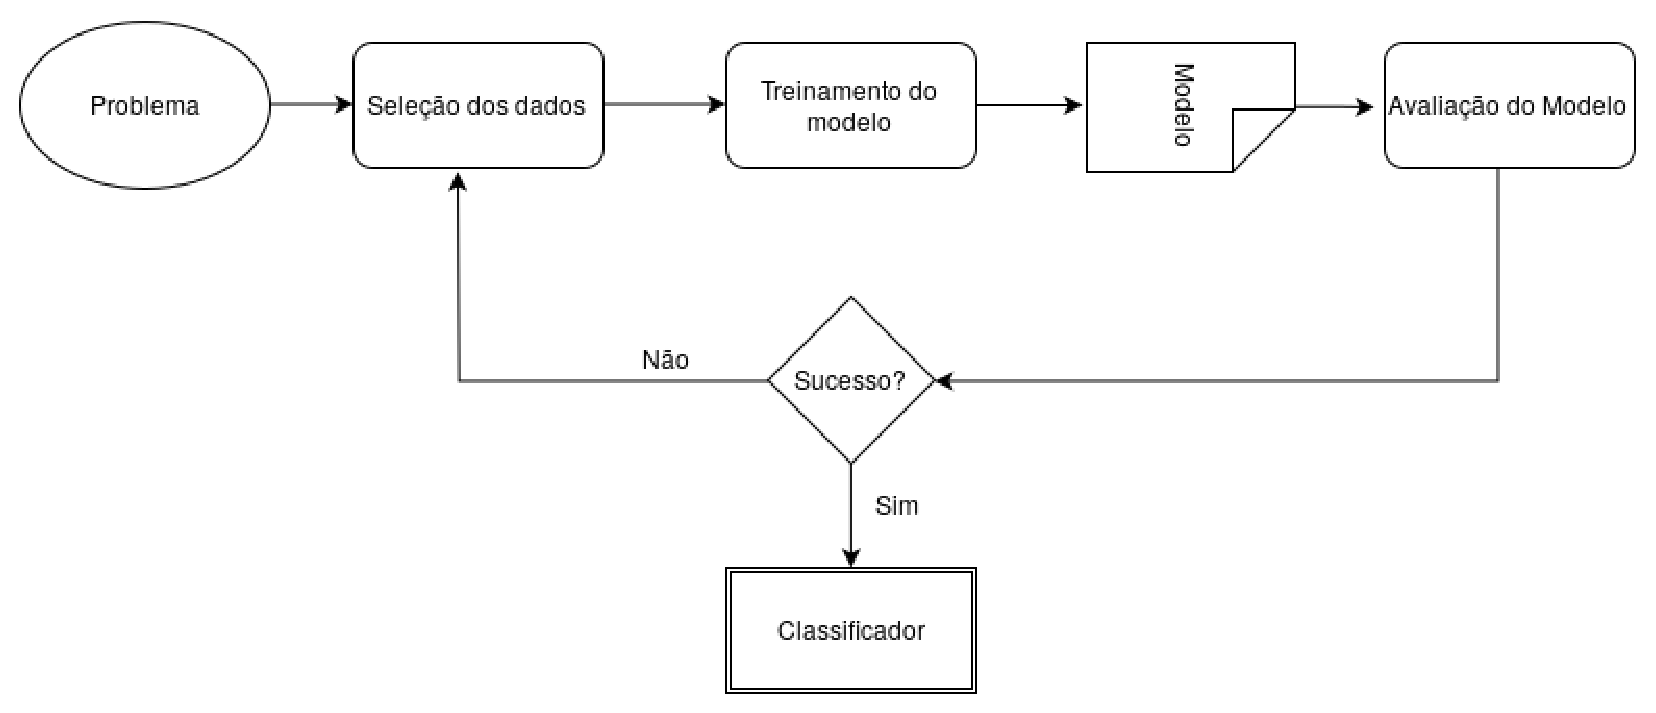
\includegraphics[width=0.8\columnwidth]{fundamentacao/workflow_predictedLearning} 
  \caption{Processo de construção de um classificador em aprendizado supervisionado. Baseado em \cite{Kotsiantis:2007} e proft\footnotemark.}
  \label{fig:slclassification}
\end{figure}
\footnotetext{\url{http://en.proft.me/2015/12/24/types-machine-learning-algorithms}}

\begin{enumerate}
\item Problema: primeiramente se deve saber qual problema quer resolver.
\item Seleção dos dados: coleta do conjunto de dados (\textit{dataset}). Se existir uma pessoa com alto conhecimento sobre os atributos, este pode sugestionar quais atributos são mais significativos para o problema. Caso contrário o mais simples método é mensurar todos os atributos na esperança que as características corretas possam ser isoladas \cite{Kotsiantis:2007}.
\item Treinamento do modelo: treina-se o dataset da etapa anterior sobre um algoritmo de classificação (árvores de decisão, \textit{Fisher’s linear discriminants}, redes neurais - \textit{Multi Layer Perceptron (MLP)} \cite{Michie:1994}). Então obtêm-se um modelo, que é o algoritmo de classificação treinado com o dataset.
\item Avaliação do Modelo: é baseada em métodos avaliativos (ver seção \ref{subsec:evaluationMethods}), os quais têm o propósito de verificar a generalização do modelo, ou seja, verificar o quão bom é o modelo do classificador quando submetido a instâncias desconhecidas (que não fazem parte do modelo). Uma das medidas utilizadas por tais métodos é a taxa de acurácia (percentagem das predições feitas corretamente dividida pelo número total de predições realizadas) \cite{Kotsiantis:2007}.
\item Classificador: se o modelo foi validado na etapa anterior, este generaliza o suficiente para o problema proposto, então este modelo pode ser utilizado como o classificador final (pode ser implantado em um sistema), caso contrário reinicia-se o processo a partir da ``seleção de dados'' reavaliando as decisões de cada etapa.
\end{enumerate}

Dentre os algoritmos citados na etapa de treinamento da Figura \ref{fig:slclassification}, as redes neurais são modelos que atendem bem tanto problemas de classificação que não são linearmente separáveis (problemas que se adequam mais a realidade), quanto problemas que são linearmente seperáveis, entretanto, utilizar-se das redes neurais para problemas linearmente separáveis é totalmente desaconselhável, já que pode ser muito mais custoso computacionalmente.\cite{Zhang:2000}\cite{Elizondo:2006} A Figura \ref{fig:slseparablenonseparable} ilustra problema linearmente separável e problema não separável linearmente. Apesar de alguns problemas serem não linearmente separáveis, estes podem ser separados de forma linear sem perdas substânciais (Figura \ref{fig:eixos_4_atributos}).

Algumas comparações \cite{Firdausi:2010, Arora:2012, Karthikeyan:2013} vêm sendo realizadas entre J48 (árvore de decisão, implementação WEKA \cite{Hall:2009}) e MLP (rede neural). Nestas, J48 obteve resultados melhores ou próximos para problemas de classificação binária (entre duas classes) e mostrou-se ser muito menos custoso computacionalmente. Sendo assim, o uso do algoritmo J48 (seção \ref{subsec:j48}) parece ser uma boa escolha e, este será utilizado como base do \textit{DECORATE}, ver seção \ref{subsec:decoration}, o qual será o método de classificação utilizado neste trabalho.

\begin{figure}[!htb] \centering 
  \centering
  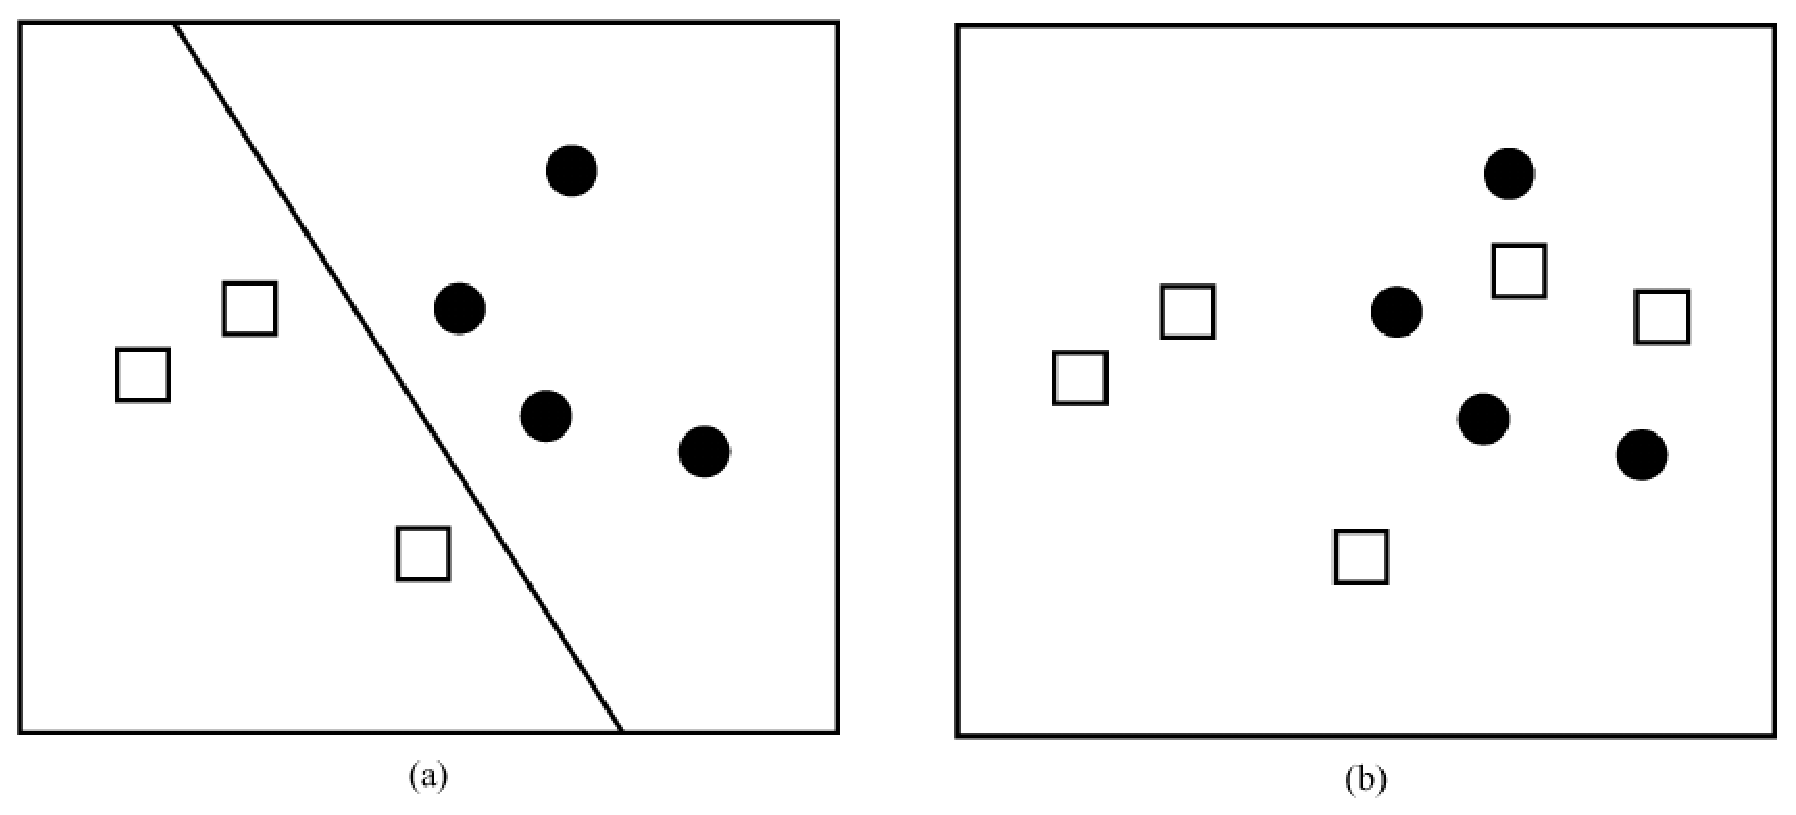
\includegraphics[width=0.8\columnwidth]{fundamentacao/linear_and_nonLinear} 
  \caption{(a) Problema linearmente separável. (b) Problema não separável linearmente. \cite{Elizondo:2006}} 
  \label{fig:slseparablenonseparable}
\end{figure}

\subsection{J48}
\label{subsec:j48}
**

\subsection{DECORATE - um método \textit{ensemble}}
\label{subsec:decoration}
Um método \textit{ensemble} combina as decisões de diversos classificadores para chegar numa decisão final. A diversidade das hipotéses dos classificadores do \textit{ensemble} é tida como um importante fator para obter uma boa generalização. O DECORATE \textit{(Diverse Ensemble Creation by Oppositional Relabeling of Artificial Training Examples)} constrói diversas hipóteses utilizando datasets de treino adicionais gerados artificialmente. Resultados experimentais demonstraram que o DECORATE tendo como algoritmo base o J48 coseguiu obter taxas de acurácia satisfatórias, mais altas que outros métodos \textit{ensemble} e, melhores do que se o J48 fosse utilizado de forma isolada. O DECORATE também se saiu muito bem em \textit{datasets} pequenos, nos quais obteve um bom grau de generalização \cite{Melville:2003, Melville:2004}.

No DECORATE, o \textit{ensemble} é gerado de forma iterativa, ou seja, a cada iteração é gerado um classificador e este é adicionado ao \textit{ensemble}. Na primeira iteração o \textit{ensemble} contém o classificador treinado no \textit{dataset} original. A partir da segunda iteração os classificadores são gerados com o \textit{dataset} original mais dados artificiais. O número de exemplos artificiais a serem gerados é especificado como um fator em cima do tamanho do \textit{dataset} de treino. Caso a adição do novo classificador ao \textit{ensemble} aumente sua taxa de erro, este é ignorado, senão é adicionado ao \textit{ensemble}. Este procedimento é repetido até que se alcance um número de \textit{committee} (membro do comitê julgador ou classificador) desejado ou exceda o limite de iterações \cite{Melville:2003}.

Para classificar um exemplo não rotulado, $x$, utiliza-se a seguinte fórmula \ref{eq:decorate}, onde $C_{i}$ é um classificador pertencente ao \textit{ensemble} $C^*$, $|C^*|$ representa a quantidade de classificadores no \textit{ensemble} e $P_{C_{i,y}}(x)$ é a probabilidade de $x$ pertencer a classe $y$ de acordo com o classificador $C_{i}$.

\begin{equation}
  P_{y}(x) = \frac{\sum_{C_{i} \in C^*}P_{C_{i,y}}(x)}{|C^*|}
  \label{eq:decorate}
\end{equation}

**colocar formula maxima probabilidade
**explicar como é gerado o dataset artificial

\subsection{Métodos avaliativos}
\label{subsec:evaluationMethods}
Métodos avaliativos têm o propósito de verificar a generalização do modelo, ou seja, verificar quão bom é o modelo do classificador quando submetido a instâncias desconhecidas (que não fazem parte do modelo). Para isto, utiliza-se de medidas estatísticas para auxiliar na tarefa \cite{Witten:2005}. Como por exemplo, acurácia, \textit{precision}, \textit{recall}, dentre outras. As medidas estatísticas citadas são baseadas em quatro componentes: verdadeiro positivo (\textit{True Positive - TP}), verdadeiro negativo (\textit{True Negative - TN}), falso positivo (\textit{False Positive- FP}) e falso negativo (\textit{False Negative- FN}) \cite{Davis:2006}.

\begin{itemize}
\item Verdadeiro positivo (TP): instância que pertence a classe positiva e que foi corretamente classificada como positiva.
\item Verdadeiro negativo (TN): instância que pertence a classe negativa e que foi classificada corretamente como negativa.
\item Falso positivo (FP): instância que pertence a classe negativa e que foi classificada  incorretamente como positiva.
\item Falso negativo (FN): instância que pertence a classe positiva e que foi classificada incorretamente como negativa.
\end{itemize}

\begin{itemize}
\item \textit{Accuracy}: taxa correta de classificação em relação a todos os exemplos, a qual pode ser visualizada e obtida através da fórmula \ref{eq:accuracy} \cite{Metz:1978}.
\item \textit{Precision}: mede a taxa de exemplos classificados como positivos que realmente são positivos. Ou seja, dentre todos os exemplos classificados como positivos, quais realmente são positivos? Esta relação pode ser visualizada e obtida através da fórmula \ref{eq:precision} \cite{Davis:2006}.
\item \textit{Recall} ou \textit{True Positive Rate - TPR}: mede a taxa de exemplos positivos que foram corretamente classificados. Ou seja, dentre os exemplos classificados como positivos (que realmente são positivos) e os classificados como negativos (mas que são positivos), qual a taxa de exemplos positivos classificados corretamente?  Esta relação pode ser visualizada e obtida através da fórmula \ref{eq:recall} \cite{Davis:2006}.
\end{itemize}

\begin{equation} 
  Accuracy = \frac{TP+TN}{TP+TN+FP+FN} 
  \label{eq:accuracy}
\end{equation}

\begin{equation} 
  Precision = \frac{TP}{TP+FP}
  \label{eq:precision}
\end{equation}

\begin{equation} 
  Recall = \frac{TP}{TP+FN} 
  \label{eq:recall}
\end{equation}

Outra medida utilizada é o desvio padrão, utilizada para verificar a dispersão de um conjunto de dados medido, por exemplo, o desvio padrão de cada conjunto das medidas avaliativas citadas anteriormente (\textit{Precision}, \textit{Recall}, \textit{Accuracy}) quando aplicado o \textit{stratified-k-fold-cross-validation}. Um desvio padrão baixo indica que os elementos do conjunto têm valores próximos ao esperado, enquanto que valores altos indicam que os elementos estão dispersos dentro de uma faixa grande de valores \cite{Kerr:2002}, \cite{Bland:1996}.

O desvio padrão pode ser medido de acordo com a fórmula \ref{eq:standarddev}, que é a $\sqrt{variância}$. Onde $x_{i}$ é um elemento do conjunto, $\bar{x}$ é a média aritmética dos \textit{i} elementos, e \textit{n} é a quantidade de elementos do conjunto. Usualmente o desvio padrão é também calculado para somente um subconjunto das medidas, desta forma o valor produzido é uma estimativa do desvio padrão para a população dos dados em questão. Para este caso em específico, a fórmula \ref{eq:standarddev} sofre uma pequena alteração (fórmula \ref{eq:standarddevsub}, ao  invés de \textit{n}, tem-se \textit{n-1}), a fim de corrigir os possíveis erros gerados por tal estimativa \cite{Kerr:2002}.

\begin{equation} 
  Desvio~padrão~(S) = \sqrt{\frac{\sum{(x_{i}-\bar{x})^2}}{n}} 
  \label{eq:standarddev}
\end{equation}

\begin{equation} 
  Desvio~padrão~(S) = \sqrt{\frac{\sum{(x_{i}-\bar{x})^2}}{n-1}} 
  \label{eq:standarddevsub}
\end{equation}

Uma exemplificação da mensuração do desvio padrão pode ser realizada com os dados da Tabela \ref{table:datakcrossvalidation} e aplicação da fórmula \ref{eq:standarddev}. Os elementos \textit{$x_{i}$} (\textit{recall}) da população foram gerados utilizando \textit{stratified-10-fold-cross-validation} em cima de um dos \textit{datasets} gerados através de tetes iniciais realizados neste trabalho com o classificador MLP. A soma dos \textit{$x_{i}-\bar{x}$}, na segunda coluna da tabela, gerou um valor diferente de zero devido a aproximação realizada para duas casas decimais, o correto seria 0 (zero). A aplicação da fórmula neste cenário pode ser visualizada em \ref{eq:standarddevapli}.

\begin{equation} 
  Desvio~padrão~(S) = \sqrt{\frac{\sum{(x_{i}-\bar{x})^2}}{n}}=\sqrt{\frac{4173.42}{10}}=24.43\%
  \label{eq:standarddevapli}
\end{equation}

\begin{table}[!htp]
  \centering
  \begin{tabular}{|c c c|}
    \hline
       {\bf $x_{i}$(\%)} & {\bf $x_{i}-\bar{x}$(\%)} & {\bf $(x_{i}-\bar{x})^2$(\%)$^2$} \\
    \hline
       100.00 & 19.17 & 367.49\\
    \hline
       66.67 & −14.16 &  200.50\\
     \hline
       100.00 & 19.17 & 367.49\\
    \hline
       100.00 & 19.17 & 367.49\\
     \hline
       75.00 & −5.83 & 33.99\\
    \hline
       100.00 & 19.17 & 367.49\\
     \hline
       66.67 & −14.16 & 200.50\\
    \hline
       50.00 & −30.83 & 950.49\\
     \hline
       50.00 & −30.83 &  950.49\\
    \hline
       100.00 & 19.17 & 367.49\\
    \hline\hline
       $\sum=$808.34 & 0.04 &  4173.42\\
    \hline
  \end{tabular}
  \caption{Medidas \textit{recall} mensuradas a partir da aplicação da técnica \textit{stratified-10-fold-cross-validation} com o classificador MLP sobre um dos \textit{datasets} gerados nos testes iniciais deste trabalho. Tabela baseada em \cite{Kerr:2002}.}
  \label{table:datakcrossvalidation}
\end{table}
                    
Um método bastante simples para avaliar um modelo é dividir o dateset em dois grandes conjuntos (um para a construção do modelo - treino, e outro para testar o modelo - teste). Então se faz pelo menos uma medição estatística (por exemplo, acurácia) de cada instância do \textit{dataset} de teste. Assim, pode-se utilizar o mesmo procedimento com outro modelo e realizar comparações. Mas esta técnica só é aceitável quando se tem um conjunto de dados grande o suficiente para realizar este tipo de repartição \cite{Kotsiantis:2007}. Quando não se tem um dataset de tamanho avantajado, recorre-se a outros tipos de métodos para verificar a generalização do modelo, tais como, \textit{randomized-holdout} e \textit{stratified-k-fold-cross-validation} \cite{Witten:2005}.

No método \textit{randomized-holdout} uma parte do dataset é escolhida randomicamente para treino e o restante é utilizado para teste, normalmente considerando a proporção de dois terço (treino) e o restante para teste. Este processo então é repetido diversas vezes e é computada a média das medidas estátisticas de cada repetição. Em cada repetição deve-se randomizar o dataset de maneira distinta \cite{Witten:2005}.

No método \textit{stratified-k-fold-cross-validation} é escolhido um número fixo k de \textit{folds} (compartimentos ou pastas). O \textit{dataset} é dividido randomicamente em k pastas iguais (ou aproximadamente), nas quais cada classe é representada aproximadamente na mesma proporção (estratificação - preserva a representatividade dos dados). 
Um compartimento é então utilizado para teste e, os k-1 restante são utilizado para treino, como pode-se observar na Figura \ref{fig:kfoldcrossvalidation}. Daí computa-se uma medida estatística. Então o procedimento é executado k vezes. Por fim têm-se uma media das medidas estatísticas das k repetições. Assim como no \textit{randomized-holdout} é recomendável que se repita o \textit{stratified-k-fold-cross-validation} diversas vezes, com randomização diferente para cada repetição. Este método é um dos mais utilizados quando se tem uma base de dados pequena \cite{Witten:2005}.

\begin{figure}[!htb] \centering 
  \centering
  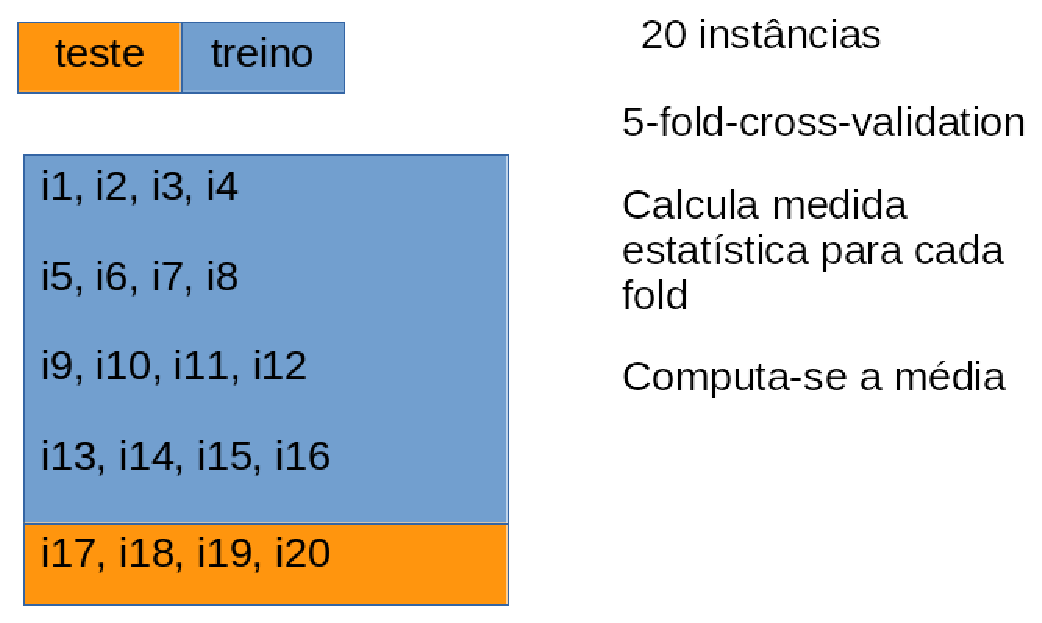
\includegraphics[width=0.8\columnwidth]{fundamentacao/k-fold-crossvalidation} 
  \caption{k-fold-cross-validation. Adaptado de \cite{Olson:2008}.} 
  \label{fig:kfoldcrossvalidation}
\end{figure}

Normalmente para o valor de k, no método descrito anteriormente, utiliza-se k=10. Este número de k tornou-se padrão após uma quantidade enorme de testes em datasets utilizando diferentes técnicas de classificação, os quais demonstraram k=10 como sendo aproximadamente a melhor escolha. A mesma quantidade (dez) têm sido escolhida como padrão para o número de repetições do \textit{stratified-k-fold-cross-validation} \cite{Witten:2005}.

No próximo capítulo será apresentada a proposta...***
